\documentclass[a4paper,12pt]{report}

\usepackage[a4paper]{geometry}
\geometry{left=3.5cm,right=2.5cm,top=3cm,bottom=3cm} % proposition

\usepackage[latin1]{inputenc}
\usepackage[T1]{fontenc}

%\usepackage{lipsum} %Pour faire des essais

\usepackage[english,francais]{babel}

\usepackage{lmodern}
\rmfamily \DeclareFontShape{T1}{lmr}{b}{sc}{<->ssub*cmr/bx/sc}{}
\DeclareFontShape{T1}{lmr}{bx}{sc}{<->ssub*cmr/bx/sc}{}

\usepackage{amssymb,amsmath,amsthm,amscd}
\usepackage[all]{xy}
\usepackage{mathrsfs}
\usepackage{subfig}

\usepackage{float}
\usepackage{rotating}


\usepackage{tabularx}
\usepackage{calc}
\usepackage{graphicx}
\usepackage[colorlinks=true,linkcolor=blue]{hyperref}

\usepackage[francais]{babel}
\usepackage{amsfonts}
\usepackage{latexsym}
\usepackage{makeidx}
\usepackage{color}
\usepackage{xcolor}
\usepackage{fancyhdr}
\usepackage{stmaryrd}
\usepackage{fancybox}
%\pagestyle{fancy}
\pagestyle{fancy}
\fancyhf{}
\fancyhead[LE,RO]{\thepage}
\fancyhead[RE,LO]{\rightmark}
\fancyfoot[CE,LO]{\leftmark}
\fancyfoot[LE,RO]{\thepage}
\renewcommand{\footrulewidth}{1pt}

\usepackage{minitoc}%pour utiliser les mini table of contenent
\usepackage{setspace}
\renewcommand{\baselinestretch}{ 1.3}
 \setcounter{secnumdepth}{4}
\setcounter{tocdepth}{4}
\usepackage[Lenny]{fncychap}

\renewcommand{\theequation}{\thechapter.\arabic{equation}}
\newtheorem*{thm*}{Th�or�me}
\newtheorem*{rem*}{Remarque}
\newtheorem{definition}{Definition}[chapter]
\newtheorem{defn}{D�finition}[chapter]
\newtheorem{theorem}{Theorem}[chapter]
\newtheorem{lemma}{Lemma}[chapter]
\newtheorem{proposition}{Proposition}[chapter]
\newtheorem{corollary}{Corollary}[chapter]
\newtheorem{remark}{Remark}[chapter]
\newtheorem{thm}{Th�or�me}[chapter]
\newtheorem{ep}{Exemple}[chapter]
\newtheorem{lemme}{Lemme}[chapter]
\newtheorem{rem}{Remarque}[chapter]
\newtheorem{pro}{Propri�t�}[chapter]
\newtheorem{prf}{Preuve}[chapter]
\newcommand{\ree}{\mathbb{R}}
\newcommand{\x}{\mathbb{X}}
\newcommand{\z}{\mathbb{Z}}
\newcommand{\s}{\mathcal{S}}
\newcommand{\cc}{\mathcal{C}}
\newcommand{\f}{\mathcal{F}}
\newcommand{\g}{\mathcal{G}}
\newcommand{\m}{\mathbb{M}}
%%%%%%%%%%%%%%%%%%%%%%%%%%%%%%%%%%%%%%%%%%%%%%%%%%%%%%%%%%%%%%%%%%%%%%%%%%%%%%%%%%

\usepackage[automake]{glossaries} %Load glossaries package
\makeglossaries
%%%%%%%%%%%%%%%%%%%%%%%%%%%%%%%%%%%%%%%%%%%%%%%%%%%%%%%%%%%%%%%%%%%%%%%%%%%%%%%%%%

%==========================================================================================================
% =========================== Commandes diverses ===============================
\makeatletter
\setlength{\@fptop}{0pt}
\makeatother
%\input{macros}
%\input{macrosmath}

% List des Abrreviations
\newglossaryentry{MVP}{name={MVP},description={Minimum Viable Product}}
\newglossaryentry{PFE}{name={PFE},description={Projet de Fin d'\'Etude}}
\newglossaryentry{OCP}{name={OCP},description={Office Ch\'erifien des Phosphates}}
\newglossaryentry{LDAP}{name={LDAP},description={Lightweight Directory Access Protocol}}
\newglossaryentry{AD}{name={AD},description={Active Directory}}
\newglossaryentry{NFS}{name={NFS},description={Network File System}}
\newglossaryentry{ERD}{name={ERD},description={Entity relationship diagram}}
\newglossaryentry{API}{name={API},description={Application programming interface}}
\newglossaryentry{MVC}{name={MVC},description={Model View Controller}}
\newglossaryentry{MVP1}{name={MVP},description={Model View Presenter}}
\newglossaryentry{REST}{name={REST},description={Representational state transfer}}
\newglossaryentry{DF}{name={DF},description={Digital Factory}}
\newglossaryentry{HTTP}{name={HTTP},description={HyperText Transfer Protocol}}
\newglossaryentry{NAS}{name={NAS},description={Networked Attached Storage}}
\newglossaryentry{SMS}{name={SMS},description={Short Message Service}}
\newglossaryentry{JWT}{name={JWT},description={JSON Web Token}}
\newglossaryentry{SQL}{name={SQL},description={Structured Query Language}}







\begin{document}

\selectlanguage{french}


\addtocounter{page}{-1}
%\include{pagedegarde}
\pdfbookmark[0]{Page de garde}{garde}
% La commande pdfbookmark permet � hyperref d'ajouter la page de garde dans le
% menu du fichier compil� (dvi, pdf)

\thispagestyle{empty}
% pour ne pas avoir de num�ro de page sur la page de garde -- le compteur de
% page est cependant � 1, c'est-�-dire que la num�rotation commence � partir
% de la page de garde

\begin{center}
  \begin{tabularx}{\textwidth}{m{1.5cm}Xm{1.5cm}X}
    
\includegraphics[width = 3cm]{Figures/usms}
    & \begin{center}{\textbf{ Universit� Sultan Moulay Slimane}\\
{\textbf{Ecole Nationale des Sciences Appliqu�es -Khouribga-}}}

 \vspace{\stretch{2}}% Permet de cr�er un espace vertical de longueur variable (\stretch) et de "poids" 2

\end{center}
       & 
\includegraphics[width =3cm]{Figures/logo1bis}\\
  \end{tabularx}
\end{center}
%%\hspace{\stretch{2}}\boxed{N� d'ordre: 05/2018}
\begin{center}



\vspace{\stretch{1}} \textbf{Projet de fin d'�tude} 


En vue de l'obtention du dipl�me 

\vspace{\stretch{2}}
{\Huge \textsc{INGENIEUR D'ETAT}}\\
\textbf{Fili�re : G�nie Informatique }

\vspace{\stretch{2}}
\textbf{Pr�sent� par}\\
\textbf{Bahaa Eddine ELBAGHAZAOUI } 

\vspace{\stretch{2}}

\hrule \vspace{\stretch{1}} {\LARGE \textbf{Contribution \`a la r\'ealisation de la plateforme Prospektor}} \vspace{\stretch{1}} \hrule
\vspace{\stretch{1}}


\vspace{\stretch{2}}

Soutenu le  (date de soutenance), devant le jury :

\vspace{\stretch{2}} {\Large
\begin{tabular}{lll}
\small NOM 1 &\small �tablissement  &\small Pr�sident\\
\small NOM 2 &\small �tablissement  &\small Examinateur\\
\small NOM 3 &\small �tablissement  &\small Examinateur\\
\small Abdelhaq ELABI &\small Groupe OCP  &\small Encadrant Externe\\
\small Mohamed AMNAI &\small ENSA-K  &\small Encadrant Interne\\
\end{tabular}
}

\end{center}

\cleardoublepage % pour laisser une page blanche au verso de la page de garde


\newpage
\newpage
  \chapter*{Remerciements}


%%%%%%%%%%%%%%%%%%%%%%%%%%%%%%%%%%%%%%%%%%%%%%%%%%%%%%%%%%%%%%%%%%%%%%%%%%%%%%%%%%%%%%%%%%%%\chapter*{Remerciements}




%\newpage
% \include{r�sum�}
%%%%%%%%%%%%%%%%%%%%%%%%%%%%%%%%%%%%%%%%%%%%%%%%%%%%%%%%%%%%%%%%%%%%%%%%%%%%%%%%%%%%%%%%%%%%%%%%%%%%�\include{r�sum�}

\setcounter{tocdepth}{2} 
\pdfbookmark[0]{Table des mati�res}{tablematieres}
%%%%%%%%%%%%%%%%%%%%%%%%%%%%%%%%%%%%%%%%%%%%%%%%%%%%%%%%%%%%%%%%%%%%%%%%%%%%%%%%%%%%%%%%%%%%%�\include{pr�sentation}

\tableofcontents
\listoffigures

\printglossary[title={List of Abbreviations}] %Generate List of Abbreviations


\chapter{Introduction}


La gestion des activit\'es m\'etiers devient de plus en plus un d\'efi majeur pour les soci\'et\'es, un d\'efi qui est aujourd'hui un point d\'eterminant en termes d'optimisation des processus m\'etiers ainsi que l'am\'elioration de leur visibilit\'e et de leur gestion. Les entreprises manufacturi\`eres changent de strat\'egie au fur et \`a mesure de l'\'evolution des march\'es. Soumises \`a de fortes pressions concurrentielles au cours des derni\`eres d\'ecennies, les industries se sont orient\'ees vers la digitalisation.

Dans ce cadre-l\`a s'inscrit le sujet de mon \gls{PFE} au sein de l'\gls{OCP}, dont le but est de concevoir et impl\'ementer une solution informatique avec une architecture moderne pour digitaliser le processus m\'etier. Dans notre situation est gestionn\'e les anomalies dans les sites de group \gls{OCP}.

Le point de d\'epart de notre projet est de faire une analyse profonde pour r\'ealiser la premi\`ere version \gls{MVP} ( Une r\'ealisation qu'on peut la mettre en face des clients pour commencer \`a valider nos hypoth\'eses), apr\`es on va faire des am\'eliorations correspondants aux nos besoins. L'\'equipe  travaille avec une m\'ethodologie Scrum selon les Epics trac\'es dans la RoadMap du projet.

Le pr\'esent rapport d\'ecrit l'ensemble du travail r\'ealis\'e dans le cadre de ce projet, il contient quatre chapitres. Le premier chapitre contient une description du contexte g\'en\'eral du projet notamment la pr\'esentation de la Digital Factory de l'\gls{OCP} ainsi que la motivation et les objectifs du projet. Le deuxid\`eme chapitre pr\'esente une analyse de besoins fonctionnels et non fonctionnels. Par la suite le troisid\`eme chapitre mettra l'accent sur l'ensemble des \'el\'ements de l'\'etude conceptuelle. Enfin, le chapitre quatre pr\'esentera les r\'esultats de l'impl\'ementation.
\chapter{Contexte g\'en\'eral}
\section{Introduction}
Ce chapitre abordera comme sujet la situation du contexte g\'en\'eral du projet, sur un niveau organisationnel en pr\'esentant l'organisme d'accueil, et sur un niveau contextuel qui refl\`ete la motivation et les objectifs du projet ainsi que la m\'ethodologie de travail durant son d\'eroulement.
\section{Pr\'esentation de l'organisme d'accueil}

\subsection{Office ch\'erifien des phosphates}

L'Office Ch\'erifien des Phosphates \`a sa cr\'eation, le Groupe OCP, depuis 1975, a \'evolu\'e sur le plan juridique, pour devenir en 2008 une soci\'et\'e anonyme d\'enomm\'ee ${\triangleleft}$ OCP S.A ${\triangleright}$.

D'une activit\'e d'extraction et de traitement de la roche \`a ses d\'ebuts, OCP s'est positionn\'e au fil du temps sur tous les maillons de la chaine de valeur, de la production d'engrais \`a celle d'acide phosphorique, en passant par les produits d\'eriv\'es. L'OCP trouve, depuis sa cr\'eation, les ressources de sa croissance continue et de son leadership dans sa strat\'egie industrielle. Celle-ci est rythm\'ee par une mont\'ee en puissance r\'egulid\`ere de l'outil de production, par une politique ambitieuse de partenariats durables et servie par une politique financid\`ere efficace.

Ces partenariats touchent aussi bien des accords de livraison \`a moyen et \`a long terme que la construction d'unit\'es de production sous forme de jointventures, bas\'ees au Maroc et \`a l'\'etranger. Aujourd'hui, OCP compte douze filiales et joint-ventures ainsi que quatre bureaux de repr\'esentations dans le monde.

Depuis sa cr\'eation, OCP est pass\'e de quelques centaines de personnes \`a prd\`es de 23 000 collaborateurs et 46 milliards de DH de chiffre d'affaires en 2013.

Afin de mener \`a bien la transformation digitale du Groupe OCP, l'entit\'e ${\triangleleft}$ Digital Office ${\triangleright}$ s'organise autour des principes manag\'eriaux suivants :

\begin{itemize}
\item Flexibilit\'e et agilit\'e dans l'allocation des ressources humaines dans une logique d'efficacit\'e et ce, \`a travers une structuration en pools permettant l'agilit\'e dans le staffing, la r\'eduction des niveaux hi\'erarchiques, ainsi que le renforcement de la collaboration et de l'autonomie.
\item Ouverture forte vers les m\'etiers, dans une logique de d\'emarche centr\'ees utilisateur, par la mise en place d'interfaces m\'etiers pour capturer et challenger leurs besoins dans un objectif de cr\'eation de valeur .
\item Stimulation et accompagnement \`a l'innovation par le d\'eploiement de capacit\'es d'innovation technologique et d'acculturation digitale .
\item Synergies entre les entit\'es Digitales et celles du Systd\`eme d'Information pour concilier les besoins d'agilit\'e avec les enjeux de stabilit\'e, de s\'ecurisation et de p\'erennisation du socle SI, assurant par l\`a-même le succd\`es de la transformation.
\end{itemize}

En application de ces principes, l'entit\'e ${\triangleleft}$  Digital Office ${\triangleright}$ est structur\'ee comme suit :

\begin{itemize}
\item Une ${\triangleleft}$ {\color{orange}{Digital Factory}} ${\triangleright}$ avec des antennes sur les diff\'erents sites du Groupe, en charge de livrer les initiatives digitales de la feuille de route, dans des cycles d'it\'eration courts, \`a travers des m\'ethodes de fonctionnement agile autour d'\'equipes cross-fonctionnelles .
\item Une entit\'e ${\triangleleft}$ {\color{orange}{Syst\`emes d'Information}} ${\triangleright}$, en charge d'assurer la r\'ealisation des projets SI, le bon fonctionnement des infrastructures SI et t\'el\'ecoms du Groupe, ainsi sue l'assistance et le support aux utilisateurs du Groupe, dans le respect des exigences de qualit\'e et des meilleurs standards en la mati\`ere .
\item Une entit\'e ${\triangleleft}$ {\color{orange}{Data Management}} ${\triangleright}$ en charge d'\'elaborer une strat\'egie et un mod\`ele de gouvernance de la Data, de d\'efinir l'architecture Data sein du Groupe, et de mettre en \oe uvre les initiatives data y aff\'erentes .
\item Une entit\'e ${\triangleleft}$ {\color{orange}{Data Planning \& PMO}} ${\triangleright}$, en charge de la construction et de la mise \`a jour de la roadmap digitale du Groupe et du suivi de son ex\'ecution .
\item Une Entit\'e ${\triangleleft}$ {\color{orange}{Business Architecture}} ${\triangleright}$, en charge de conseiller et challenger les m\'etiers sur les solutions digitales pertinentes pour adresser leurs besoins, les consolider et suivre leur mise en \oe uvre .
\item Un pool ${\triangleleft}$ {\color{orange}{Digital Innovation \& Change Officers}} ${\triangleright}$, en charge d'identifier et mener des projets d'innovation en mati\`ere de Digital (veille technologique, prototypage, Open Innovation ...), ainsi que de la promotion d'une culture digitale et de nouveaux modes de travail au sein du Groupe .
\end{itemize}

\begin{figure}[!htb]
	\center{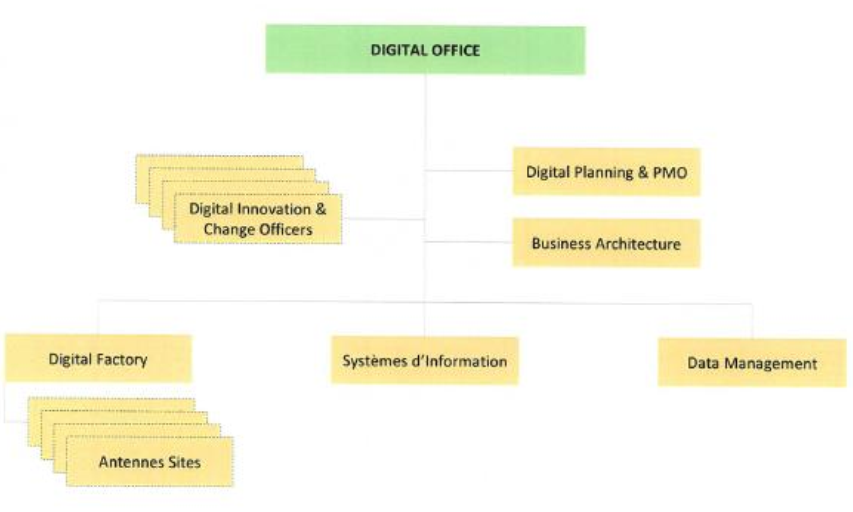
\includegraphics[width=0.8\textwidth]{Figures/digitalOffice.PNG}}
	\caption{\label{fig:my-label} Structure de la Digital Office de l'OCP}
\end{figure}

\subsection{L'importance de la digitalisation}

Le digital est un incubateur de nouveaux modes de fonctionnement \`a l'\'echelle du Groupe. Il favorise l'intrapreneuriat, la prise d'initiative et r\'einvente la mani\`ere d'interagir avec l'\'ecosyst\`eme du Groupe. Le digital repr\'esente aussi un gisement consid\'erable en termes d'innovations et de d\'eveloppement industriel et favorise l'\'emergence de nouveaux talents au sein du Groupe OCP et de son \'ecosyst\`eme.
Le challenge de cette transformation digitale r\'eside dans la diffusion d'une culture digitale aupr\`es de l'ensemble des collaborateurs et la conception de solutions innovantes pour enrichir et supporter les diff\'erents m\'etiers d'OCP.

\subsubsection{Objectifs}

\begin{itemize}
\item[\textbf{Renforcer l'efficacit\'e op\'erationnelle}]\ :anticiper les changements et agir en temps r\'eel \`a travers la promotion de l'Advanced Analytics , augmenter les capacit\'es de production, r\'eduire les co\^ots, et construire une Supply Chain agile, int\'egr\'ee et adapt\'ee \`a un march\'e dynamique.

\item[\textbf{Se connecter aux agriculteurs et aux clients}]\ :\^etre plus proches de leurs besoins, enjeux et probl\'ematiques et leur proposer des exp\'eriences ( fully digitized ).

\item[\textbf{D\'evelopper de nouveaux produits et services}]\ :augmenter la flexibilit\'e pour am\'eliorer l'existant et cr\'eer de nouvelles offres.

\item[\textbf{Explorer de nouvelles voies de croissance}]\ :introduire des m\'ethodologies de gestion de projets plus agiles, rapides et fluides, \`a travers des cycles de conception et d'innovation plus courts.
\end{itemize}

\subsection{La Digital Factory de l'OCP}

La vision digitale du Groupe OCP consiste \`a devenir un organisme de digitalisation phare de l'industrie dans la r\'egion, ainsi que et favoriser l'innovation et les moyens num\'eriques de travailler dans l'ensemble de l'organisation.

\begin{figure}[!htb]
	\center{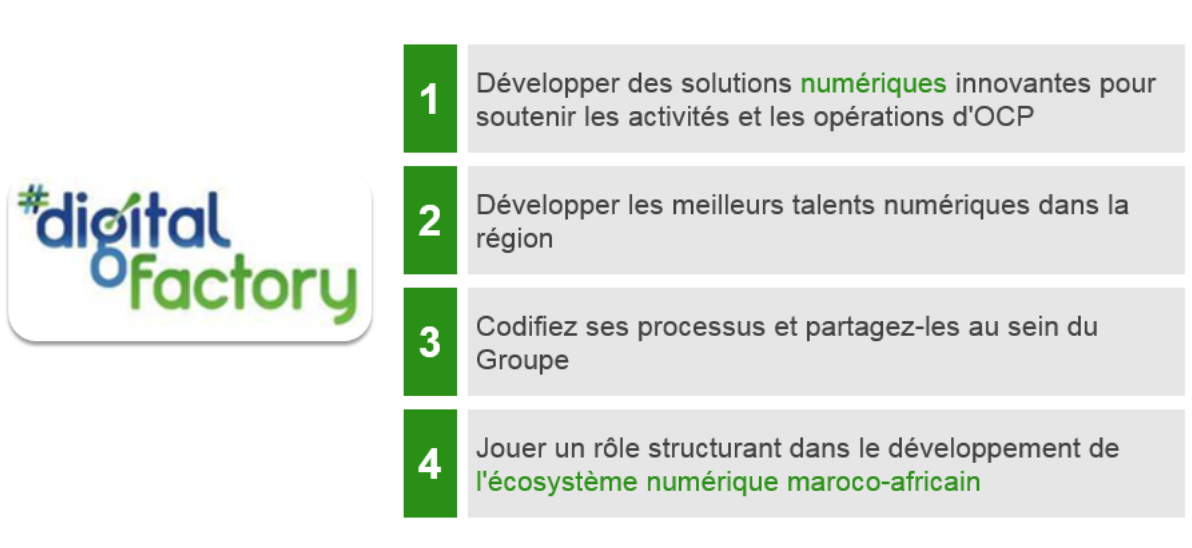
\includegraphics[width=\textwidth]{Figures/digitalFactory.PNG}}
	\caption{\label{fig:my-label} les buts majeurs de la Digital Factory de l'OCP}
\end{figure}

Le Groupe OCP a construit sa nouvelle entit\'e ${\triangleleft}$ Digital Factory ${\triangleright}$ qui sera \`a la pointe de l'innovation et de la transformation num\'erique de toute l'organisation et au-del\`a.

La Digital Factory rassemble les comp\'etences, les processus, la culture, et les points d'entr\'ees afin de mener la transformation digital et de livrer des produits digitaux. Elle vise \`a :

\begin{itemize}
\item Construire la capacit\'e interne \`a poss\'eder la d\'efinition et la livraison de produits num\'eriques
\begin{itemize}
\item R\'eduire le ${\triangleleft}$ time to market ${\triangleright}$
\item Augmenter la qualit\'e de la livraison
\item Mettre l'accent sur l'impact et les r\'esultats
\end{itemize}
\item Mettre \`a l'\'echelle une culture transformative
\begin{itemize}
\item Fournir un plan pour l'avenir du travail qui dynamise l'entreprise et encourage les employ\'es
\item Cr\'eer un vortex pour l'innovation et la cr\'eativit\'e qui attire les meilleurs talents de l'int\'erieur et de l'ext\'erieur de l'organisation
\end{itemize}
\end{itemize}

\section{Pr\'esentation g\'en\'erale du projet}
La Digital Factory de l'\gls{OCP} a entam\'e une nouvelle phase de digitalisation avanc\'ee relative au processus de gestion des anomalies. Ceci permettra aux employ\'ees d'une part d'avoir en temps r\'eel, l'ensemble des informations relatives \`a chaque \'etape du processus. Depuis l'alert du probl\`eme jusqu'\`a leur r\'esolution et d'autre part, offrira de la transparence pour \^etre plus performant et \'economiser en temps et ressources.

L'objectif g\'en\'erale du projet est de r\'ealiser une application mobile qui vas utiliser par deux types des employ\'es :
\begin{itemize}
\item Prospecteur : dont le r\^ole est d'assurer la qualit\'e / quantit\'e de phosphates en auditant les sites d'extraction.
\item Exploitant : dont le r\^ole est d'assurer la continuit\'e de l'exploitation (machines, pilotes ...).
\end{itemize}
\subsection{Pr\'esentation du projet de fin d'\'etudes}
L'extraction du phosphate dans les mines de Khouribga suivent les cinq \'etapes suivantes :

\begin{figure}[!htb]
	\center{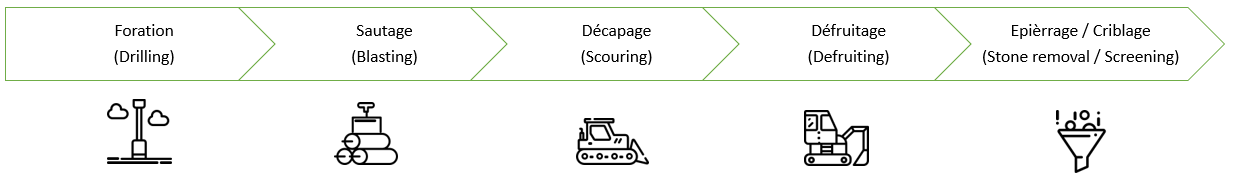
\includegraphics[width=\textwidth]{Figures/5steps.PNG}}
	\caption{\label{fig:my-label} Les cinq \'etapes d'extraction du phosphate}
\end{figure}

Les prospecteurs fournissent des informations g\'eologiques aux responsables des op\'erations (Exploitant) avant le d\'ebut du premier forage, puis suivent l'\'evolution jusqu'\`a l'extraction du phosphate.

Apr\`es le d\'ecapage, la premi\`ere couche du phosphate est visible et le prospecteur peut pr\'elever un \'echantillon pour d\'eterminer la qualit\'e du phosphate (HT: Haute Teneur, BT: Basse Teneur ...).
Disons que le premier \'echantillon pr\'elev\'e \'etait HT, mais apr\`es avoir analys\'e et stock\'e le phosphate, nous avons fait un autre test et la qualit\'e \'etait BT.

Pour \'eviter cette situation, le travail de Prospector consiste \`a assurer la qualit\'e / quantit\'e du phosphate extrait avant de le stocker et \`a \'eliminer toute anomalie en v\'erifiant et en v\'erifiant toutes les 5 \'etapes de l'extraction du phosphate.

\begin{figure}[!htb]
	\center{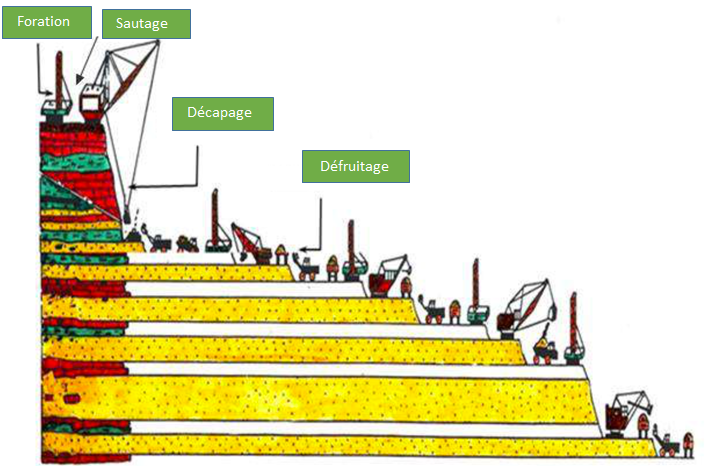
\includegraphics[width=0.8\textwidth]{Figures/levels_shema.png}}
	\caption{\label{fig:my-label} Cha\^ine cin\'etique d'extraction de phosphate}
\end{figure}

Les prospecteurs n'ont aucun support num\'erique lors de leurs inspections quotidiennes. Ils donnent toujours des instructions \`a Machine Conductors et \`a Operations Manager (Exploitant) verbalement, sans autre syst\`eme de suivi que les appels t\'el\'ephoniques ou les conversations directes.

{\color{red}{Comment pouvons-nous aider les prospecteurs \`a relever et \`a garder trace des anomalies au cours de leur inspection quotidienne pour \'eviter les souillures au phosphate?}}

\subsection{Exigences du projet}
Apr\`es une examination au terrain, les utilisateurs de notre application ont des exigences n\'ecessaires qu'on doit les impl\'ementes :
\subsubsection{Besoins des prospecteurs}
\begin{itemize}
\item S'assurer que la qualit\'e du phosphate est conforme.
\item S'assurer que le phosphate a \'et\'e completement exploit\'e
\item Communiquer facilement avec les exploitants de la mine
\item Mesurer et suivre les anomalies remont\'e lors de sa tourn\'ee.
\end{itemize}
\subsubsection{Besoins des exploitants}
\begin{itemize}
\item Terminer son shift sans incident.
\item Diriger son \'equipe avec plus d'efficacit\'e
\item Lib\'erer le chantier le plus rapidement possible
\item Veillez au respect des consignes des Prospecteurs
\item S'assurer que toutes les machines sont fonctionnelles
\end{itemize}

\subsection{Objectifs du Projet}

Les exigences initiales indiquent que la solution sera une application mobile aidant les prospecteurs et les exploitants \`a effectuer leur inspection quotidienne.

\begin{itemize}
\item R\'ep\'etition des consignes et anomalies
\item Aucun moyen de suivi des anomalies remont\'ees 
\item Disponibilit\'e de l'Exploitant sur chantier
\item Moyens de communications limit\'es entre le prospecteur et l'exploitant
\item Le t\'el\'ephone ne capte pas tou jours dans les mines 
\end{itemize}

\`A l'aide d'une s\'erie d'invites, nous pouvons r\'esoudre le probl\`eme initial et d\'efinir une feuille de route claire et coh\'erente qui nous aidera \`a d\'evelopper un MVP.

En les aidant \`a se sentir en s\'ecurit\'e et \`a \^etre productifs.

\section{Conduite du projet}
\subsection{Organisation du projet}
Apr\`es avoir pass\'e une p\'eriode de documentation et d'int\'egration au sein de la Digital Factory de l'OCP, j'ai int\'egr\'e lune \'equipe qui se constitue de 6 personnes tout en respectant la structure d'une \'equipe dans le cadre Scrum.
La figure suivante illustre l'architecture de notre \'equipe :

\begin{figure}[!htb]
	\center{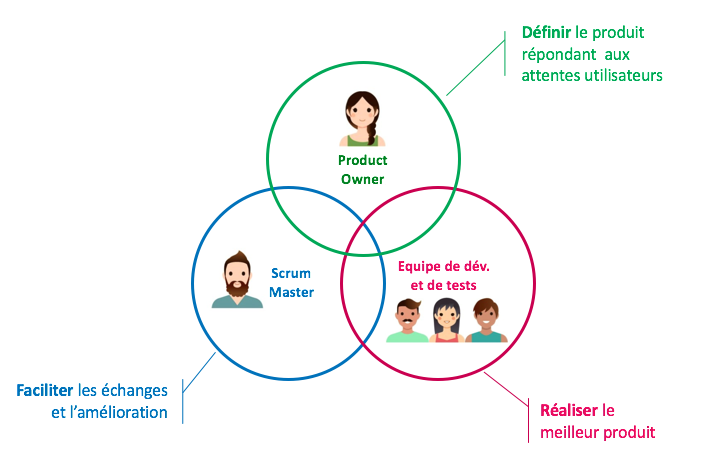
\includegraphics[width=0.8\textwidth]{Figures/scrumEquipe.png}}
	\caption{\label{fig:my-label} \'Equipe de projet}
\end{figure}

\begin{itemize}
\item Product Owner (PO),
\item 1 \'equipe de d\'eveloppement constitu\'ee de 3 d\'eveloppeurs,
\item 1 Scrum Master (SM).
\end{itemize}

Notre \'equipe Scrum est auto-organis\'ees et pluridisciplinaire. C'est \`a dire nous choisissons la meilleure fa${\c{c}}$on d'accomplir notre travail, au lieu d'\^etre dirig\'ees par des personnes externes \`a l'\'equipe.

\section{M\'ethodologie de travail}
\subsection{M\'ethodologie Scrum}
Afin de d\'erouler le projet dans des conditions standards qui s'inspirent des m\'ethodologies de travail les plus efficaces et dans le cadre de mon \'equipe de travail nous avons choisi la m\'ethodologie Scrum pour la gestion du projet.

Le choix de cette m\'ethodologie est d\^u \`a plusieurs raisons. Dans un premier temps cette m\'ethodologie favorise la productivit\'e au sein d'une \'equipe de d\'eveloppement en travaillant sur des objectifs prioritaires et \`a court terme et en suivant un d\'eveloppement it\'eratif et incr\'emental avec une planification \'evolutive bas\'ee sur la division de l'ensemble des t\^aches selon des unit\'es qu'on appelle sprint. Aussi le choix de cette m\'ethodologie tiens en compte la tendance du contexte de d\'eveloppement dans le monde qui r\'eside dans l'adaptation de l'esprit agile durant la r\'ealisation des projets, un esprit ou Scrum est l'une de ses m\'ethodologies piliers.

Le choix de Scrum comme m\'ethodologie pr\'esente plusieurs avantages li\'es \`a la productivit\'e ainsi que l'organisation du travail en se basant sur des rôles d\'efinis, ce qui n'existe pas dans les m\'ethodologies traditionnelles, qui repr\'esentent plusieurs inconv\'enients, ceux de la rigidit\'e ainsi que la g\'en\'eration massive de la documentation et la difficult\'e d'introduction des changements. Ceci justifie le choix de Scrum comme m\'ethodologie de d\'eveloppement qu'on r\'esume selon une vision d'ensemble dans la figure suivante :
\begin{figure}[!htb]
	\center{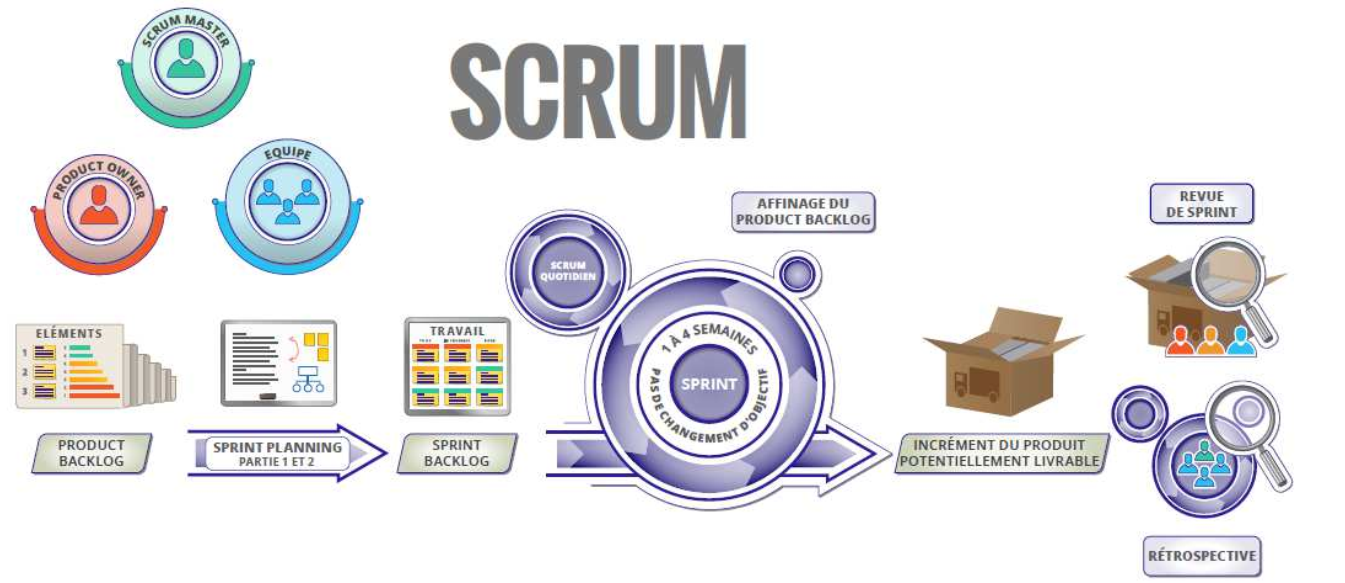
\includegraphics[width=\textwidth]{Figures/scrum.PNG}}
	\caption{\label{fig:my-label} M\'ethode SCRUM}
\end{figure}

Comme le montre la figure la r\'epartition des taches se fais selon des roles bien pr\'ecis. Dans notre cas, l'\'equipe se constitue de 8 personnes ayant les profiles suivant :
\begin{itemize}
\item[\textbf{Le PO(Product Owner)}]\ : c'est un expert m\'etier qui d\'efinit dans un premier temps les sp\'ecifications fonctionnelles. Aussi, il \'etablit la priorit\'e des fonctionnalit\'es \`a d\'evelopper ou corriger et valide les fonctionnalit\'e d\'evelopp\'ees. Bref, le PO joue le rôle du client.
\item[\textbf{Le Scrum Master}]\ : c'est expert Agile qui s'assure que les principes et les valeurs de Scrum sont respect\'es. Il assure la communication au sein de l'\'equipe ainsi que la recherche d'am\'elioration de la productivit\'e et du savoir-faire de notre \'equipe.
\item[\textbf{UX Designer}]\ : il fait le design de chaque user story selon l'exp\'erience d'utilisateur (user experience). L'UX design a plus un rôle de (conception de produit) qu'un rôle de conception graphique.
\item[\textbf{L'\'equipe de d\'eveloppement}]\ : constitu\'ee de 6 personnes qui s'occupent du d\'eveloppement des user stories ainsi que la r\'ealisation des tests unitaires et des tests d'int\'egration.
\end{itemize}


\subsection{Outils de suivi}

\subsubsection{JIRA Atlassian}

Le framework agile Scrum repose entre autres sur le principe de (transparence). Certaines informations doivent donc \^etre accessibles par tous, comme la t\^ache en cours de chacun, son \'etat d'avancement, et l'objectif actuel de l'\'equipe. D'o\`u l'importance que ces informations soient visibles en permanence.

C'est le tableau Scrum qui va jouer ce r\^ole. Il permet d'organiser le backlog, les t\^aches du sprint en cours et leur \'etat d'avancement. Les tableaux Scrum peuvent \^etre aussi simples qu'un tableau blanc et des posts-its, ou peuvent rev\^etir un format plus \'elabor\'e avec des logiciels sp\'ecialis\'es disposant de graphiques et de fonctionnalit\'es de gestion des t\^aches plus avanc\'ees.

Pour notre tableau Scrum,nous utilisons JIRA Atlasian. Notre tableau est divis\'e en 5 listes qui correspondent au flux de travail des t\^aches:

\begin{itemize}
\item \textbf{\`A Faire}: quand je planifie mon sprint, je d\'eplace les t\^aches du backlog vers cette liste.
\item \textbf{En Cours} : contient les t\^aches en cours de d\'eveloppement et de r\'ealisation.
\item \textbf{Termin\'e} : la t\^ache est compl\`ete dans la phase du d\'eveloppement mais en attente de la validation fonctionnelle par le PO
\item \textbf{Approuv\'e} : une fois la t\^ache est approuv\'ee fonctionnellement par le PO on peut la placer dans la colonne APPROUV\'E.
\item \textbf{Bloqued}: j'utilise cette liste lorsque la finalisation d'une t\^ache d\'epend d'un facteur externe (par exemple, je dois r\'ealiser un achat et obtenir l'aval de mon PO), en sp\'ecifiant les raisons du blocage dans un commentaire.
\end{itemize}

\begin{figure}[H]
	\center{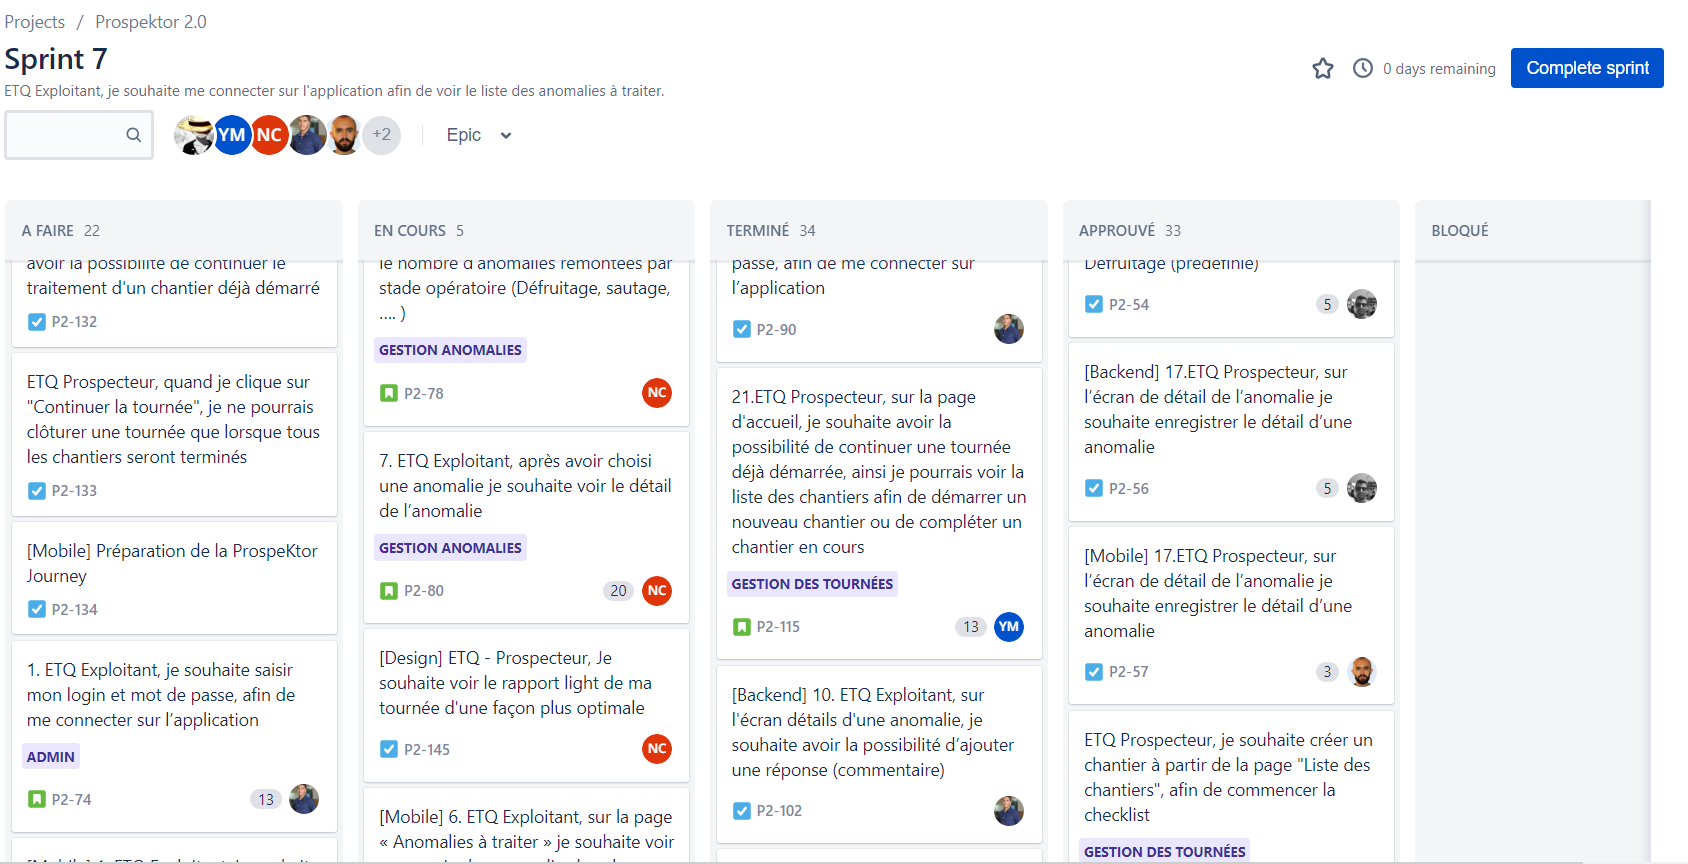
\includegraphics[width=\textwidth]{Figures/jira.png}}
	\caption{\label{fig:my-label} Capture de l'outil JIRA}
\end{figure}

\subsubsection{Slack}

Slack est une plateforme de communication collaborative sur ordinateur et smartphone. Chaque entreprise peut cr\'eer un groupe priv\'e sur Slack, et y inviter tout ou partie de ses employ\'es, qui peuvent ainsi discuter entre eux.

Avec les conversations instantan\'ees class\'ees par (cha\^ines), la communication se fluidifie, il est possible d'interagir en temps r\'eel, tout en s'adressant uniquement aux personnes concern\'ees, au contraire de l'e-mail.

L'autre atout de l'application : toutes les interconnexions qu'elle permet avec d'autres logiciels. L'outil Slack est pratique pour recevoir une notification d\`a chaque modification dans un document Drive.

\begin{figure}[H]
	\center{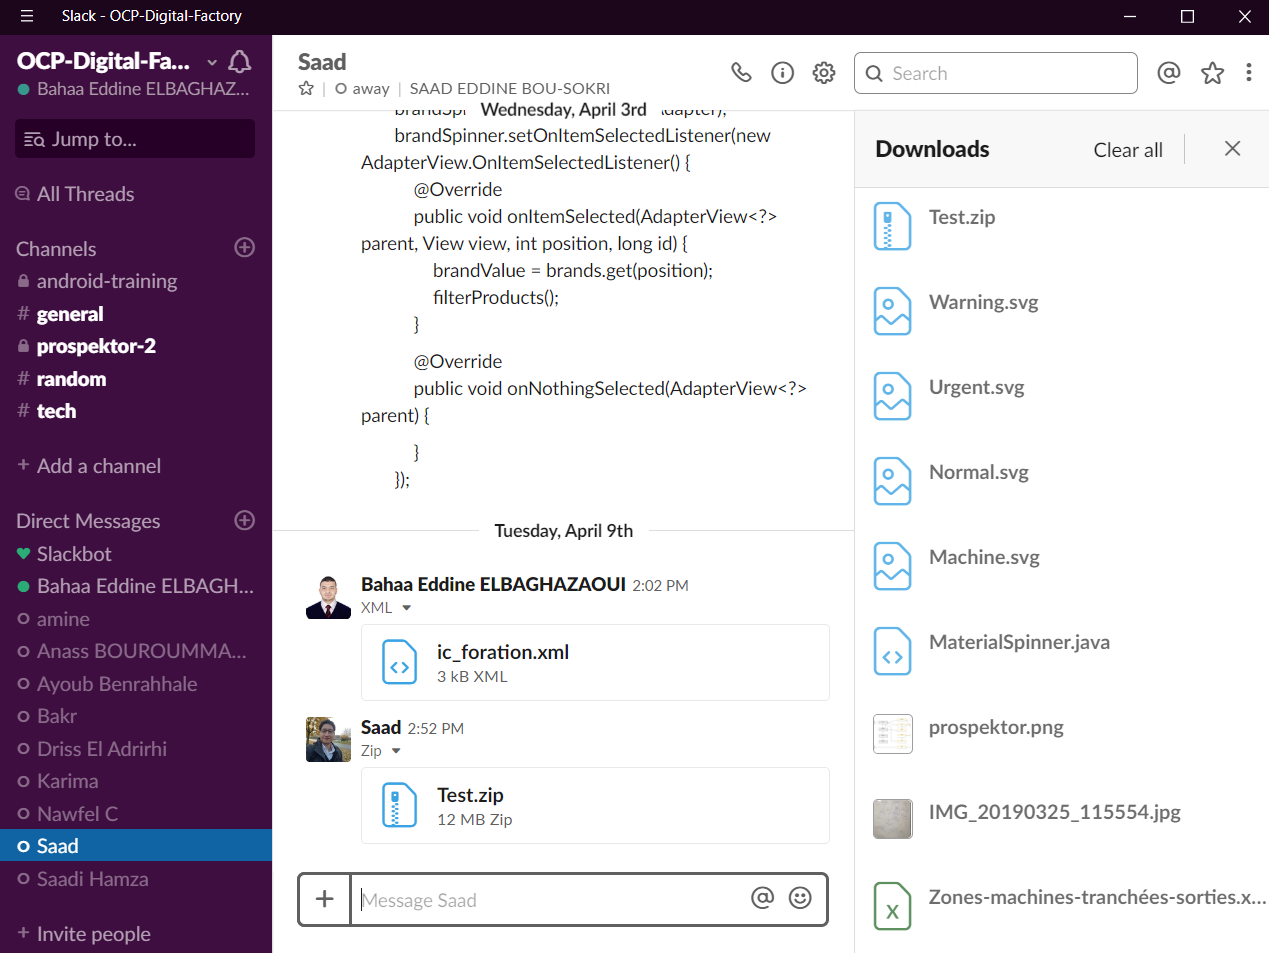
\includegraphics[width=0.5\textwidth]{Figures/slack.png}}
	\caption{\label{fig:my-label} Capture de l'outil Slack}
\end{figure}

\section{Conclusion}

Dans ce chapitre nous avons pr\'esent\'e l'ensemble des \'el\'ements qui permettent la situation de notre Projet de Fin d'\'etudes dans son contexte organisationnel ainsi que la d\'emarche de gestion du projet qui organise son d\'eroulement et les outils utilis\'es. Par la suite dans le chapitre suivant on va mettre l'accent sur l'\'etape de l'analyse et sp\'ecification des besoins qui permettra la collection des diff\'erents besoins afin de concevoir une solution qui r\'epondra aux exigences exprim\'ees
\chapter{Analyse et sp\'ecification des besoins}
\section{Introduction}
Ce chapitre est consacr\'e \`a l'analyse et \`a la sp\'ecification des besoins fonctionnels et non fonctionnels de la solution qui est une \'etape primordiale pour la r\'ealisation de notre projet.
\section{Analyse des besoins}
Dans cette partie, nous pr\'esenterons les besoins fonctionnels et non fonctionnels identifi\'es apr\`es la s\'election des besoins.
\subsection{Identification des acteurs}
Dans le cas de notre projet on consid\`ere trois acteurs :
\begin{itemize}
\item \textbf{Le prospecteur} : Il a comme mission principale de g\'erer les anomalies de la plateforme.
\item \textbf{L'exploitant} : Il permet de r\'epondre sur les anomalies qui ne sont pas encore r\'esolu.
\item \textbf{L'administrateur} : Il permet de g\'erer les  autres utilisateurs (prospecteurs, exploitants), les machines ,les g\'eolocalisation ... .
\end{itemize}
\subsection{Les besoins fonctionnels}
Au cours de cette \'etape, nous allons extraire les diff\'erentes fonctionnalit\'es offertes par notre projet.
\begin{itemize}
\item L'application \textcolor{red}{prospektor} doit permettre \`a chaque prospecteur de :
\begin{itemize}
\item suivre et consulter les anomalies qui a cr\'eer.
\item consulter la liste des attachements li\'ees par anomalies.
\end{itemize}
\item L'application \textcolor{red}{prospektor} doit permettre \`a chaque exploitant de :
\begin{itemize}
\item suivre et consulter les anomalies par \'etape, date \& criticit\'e.
\item consulter les attachements li\'ees par anomalies.
\item Ajouter des attachements aux anomalies qui ne sont pas encore r\'esolu.
\end{itemize}  
\item L'application \textcolor{red}{prospektor} doit permettre \`a chaque administrateur de :
\begin{itemize}
\item G\'erer :
\begin{itemize}
\item Prospecteurs
\item Exploitants
\item G\'eolocalisation (Mine, Zone, Tranch\'ee, Sortie)
\item Machines
\end{itemize}
\item Consulter :
\begin{itemize}
\item Tourn\'ees
\item Chantiers
\item Erreurs
\item ...
\end{itemize}

\end{itemize} 
 
\end{itemize}

\subsection{Les besoins non fonctionnels}
Outre les fonctions cit\'ees ci-dessus, l'application doit assurer en certaine mesure les caract\'eristiques suivantes :
\begin{itemize}
\item L'efficacit\'e : L'efficacit\'e de l'application doit permettre l'accomplissement de la t\^ache avec le minimum de manipulation. Ceci doit \^etre garanti pour que l'application puisse s'int\'egrer facilement dans l'environnement ou elle va \^etre d\'eploy\'ee.

\item La s\'ecurit\'e : Les diff\'erents comptes utilis\'es par les utilisateurs doivent \^etre s\'ecuris\'es et v\'erifi\'es pour \'eviter les faux comptes et les fausses informations.

\item La fiabilit\'e : Touche \`a l'aspect qualit\'e des donn\'ees et persistance des informations dans l'application ainsi que la vitesse de chargement des interfaces.
\item La performance : le temps de r\'eponse de la plateforme doit \^etre rapide.

\item La maintenabilit\'e : La solution doit \^etre stable face aux changements, ainsi qu'un fort niveau de testabilit\'e assur\'e par les tests fonctionnels.

\item La scalabilit\'e : la solution doit d'\^etre extensible en termes de la charge des requ\^etes trait\'ees.

\item L'\'evolutivit\'e : possibilit\'e d'ajout des nouvelles fonctionnalit\'es au cours du temps selon le besoin des fournisseurs.

\item Le d\'eploiement intelligent: l'introduction des nouveaux changements ne doit pas impacter les modules existants, d'o\`u le besoin d'une d\'emarche de d\'eploiement intelligente de chaque module.

\item La portabilit\'e: facilit\'e de passage d'un environnement de d\'eveloppement et tests vers un environnement de pr\'e-production ou un environnement de production.
\end{itemize} 


\subsection{Diagramme des cas d'utilisation}
Cette figure repr\'esente le diagramme de cas d'utilisation globale de l'acteur prospecteur :
\begin{figure}[H]
	\center{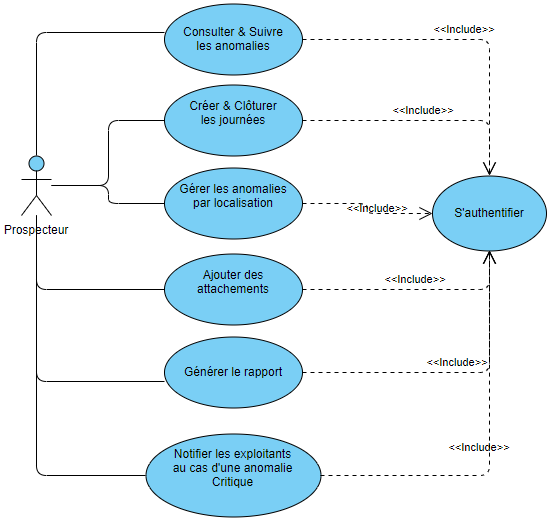
\includegraphics[width=\textwidth]{Figures/prospectorDiagram.png}}
	\caption{\label{fig:my-label} Diagramme de cas d'utilisation globale pour le prospecteur}
\end{figure}

Cette figure repr\'esente le diagramme de cas d'utilisation globale de l'acteur exploitant :
\begin{figure}[H]
	\center{\includegraphics[width=\textwidth]{Figures/exploitantDiagram.png}}
	\caption{\label{fig:my-label} Diagramme de cas d'utilisation globale pour l'exploitant}
\end{figure}

Cette figure repr\'esente le diagramme de cas d'utilisation globale de l'acteur administrateur :
\begin{figure}[H]
	\center{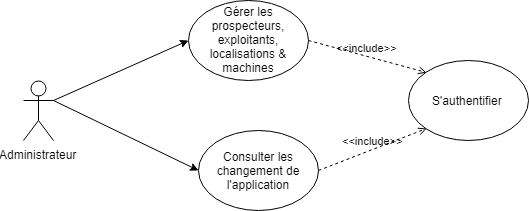
\includegraphics[width=\textwidth]{Figures/adminDiagram.png}}
	\caption{\label{fig:my-label} Diagramme de cas d'utilisation globale pour l'administrateur}
\end{figure}

\subsection{Description des cas d'utilisation}
\textbf{Prospecteur :} Les grandes \'etapes pour un prospecteur lors de l'utilisation de l'application prospektor.
\begin{itemize}
  \item Ouvrir l'application mobile prospektor
  \item S'authentifier
  \begin{itemize}
    \item Consulter les anomalies en cours de traitement
    \item Consulter les demandes d'intervention
    \item Consulter l'historique des anomalies
    \item Consulter le rapport des tourn\'ees
    \item D\'emarrer \& Continuer une tourn\'ee
    \begin{itemize}
      \item sp\'ecifier la localisation du prospection
      \item Remplir la check-list des \'el\'ements \`a auditer
      \item Cr\'eation d'une anomalie au cas d'un d\'erangement
      \item Ajouter des attachements (audio \& photos) si n\'ecessaire
    \end{itemize}
    \item Continuer la tourn\'ee vers un autre chantier
    \item Obtenir le rapport complet de la tourn\'ee 
  \end{itemize}
\end{itemize}

\textbf{Exploitant :} Les grandes \'etapes pour un exploitant lors de l'utilisation de l'application prospektor.
\begin{itemize}
  \item Ouvrir l'application mobile prospektor
  \item S'authentifier
  \begin{itemize}
    \item Consulter les anomalies en cours
    \item Consulter les anomalies \`a traiter
    \item Consulter l'historique des anomalies
  \end{itemize}
\end{itemize}

\textbf{Administrateur :} Les grandes \'etapes pour un administrateur lors de l'utilisation de l'application prospektor.
\begin{itemize}
  \item Ouvrir l'application web prospektor
  \item S'authentifier
  \begin{itemize}
    \item Consulter les utilisateurs (prospecteur \& exploitant).
    \begin{itemize}
    \item Ajouter un utilisateur.
    \item Supprimer un utilisateur.
    \item Modifier un utilisateur.
    \item D\'esactiv\'e un utilisateur.
    \item Consulter les d\'etails d'un utilisateur.
    \end{itemize}
    \item G\'erer les localisations (Mine, Zone, Tranch\'ee, Sortie).
    \item Consulter les machines.
    \begin{itemize}
    \item Ajouter une machine.
    \item Supprimer une machine.
    \item Modifier une machine.
    \item D\'esactiv\'e une machine.
    \item Consulter les d\'etails d'une machine.
    \end{itemize}
    \item Consulter les tourn\'ees.
    \item Consulter les chantiers par zones ou par \'etape.
    \item Consulter les anomalies par criticit\'e.
    \item ...

  \end{itemize}
\end{itemize}

\subsection{Exceptions des cas d'utilisation}

\textbf{Prospecteur :} Les exceptions pour un prospecteur lors de l'utilisation de l'application prospektor:
\begin{itemize}
\item Email ou mot de passe sont incorrecte.
\item Cr\'eer une anomalie sans pr\'eciser leur localisation.
\item Cr\'eer une anomalie sans description.
\item G\'en\'erer le rapport sans terminer toutes les chantiers.
\item ...
\end{itemize}
\textbf{Exploitant :} Les exceptions pour un exploitant lors de l'utilisation de l'application prospektor:
\begin{itemize}
\item Email ou mot de passe sont incorrecte.
\item Repondre \`a une anomalie sans description.
\item Repondre \`a une anomalie d\'ej\`a cl\^oturer.
\item ...
\end{itemize}
\textbf{Administrateur :} Les exceptions pour un administrateur lors de l'utilisation de l'application prospektor:
\begin{itemize}
\item Email ou mot de passe sont incorrecte
\item Ajouter un utilisateur qui n'existe pas dans le group ocp
\item Ajouter une machine sans preciser leur localisation
\item ...
\end{itemize}

\section{Planning du projet}
On a dr\'esse le RoadMap qui va \^etre r\'ealiser entre Mars et Juin sur deux parties. Chaque partie va prendre 8 semaines de travail.

Pour notre projet prospektor, On a d\'efinie 
\begin{itemize}
\item 1 Sprint = 1 Semaine
\item Daily Meeting \& check \`a 10:00 AM
\item Sprint planning chaque mercredi matin
\end{itemize}

\subsection{\gls{MVP}}
Cette version permet d'offrir une consultation compl\`ete pour le d\'eveloppement de notre produit.
\begin{figure}[H]
	\center{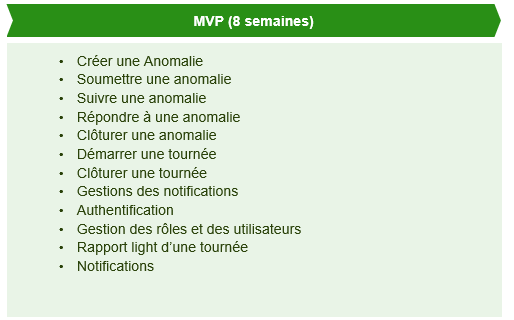
\includegraphics[width=\textwidth]{Figures/mvp.PNG}}
	\caption{\label{fig:my-label} RoadMap de la version \gls{MVP}}
\end{figure}
\subsection{Post \gls{MVP}}
Cette version est celle qui suive la premi\`ere version.
\begin{figure}[H]
	\center{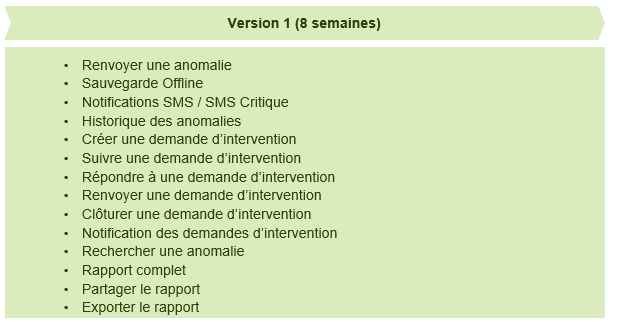
\includegraphics[width=\textwidth]{Figures/version1.PNG}}
	\caption{\label{fig:my-label} RoadMap de la version Post \gls{MVP}}
\end{figure}

 
\section{Conclusion}
Dans ce chapitre nous avons d\'etect\'e des besoins fonctionnels et non fonctionnels qui sont un compl\'ement de l'existant. Par la suite nous avons pouss\'e l'analyse des besoins vers les diagrammes de cas d'utilisation afin de visualiser les diff\'erentes fonctionnalit\'es de la solution.
\chapter{Conception g\'enerale du projet}

\section{Introduction}
Ce chapitre est consacr\'e \`a la conception g\'en\'erale du projet. Apr\`es la d\'efinition des besoins fonctionnels et non fonctionnels, nous allons passer \`a la conception de l'architecture fonctionnelle qui repr\'esente une vue globale de la solution avec une prise en consid\'eration du besoin de la modularit\'e. 

\section{Conception g\'en\'erale}

\subsection{Architecture globale du syst\`eme}

Apr\`es la d\'efinition des besoins fonctionnels et non fonctionnels, nous avons pass\'e \`a la conception de l'architecture fonctionnelle qui repr\'esente une vue globale de la solution avec une prise en consid\'eration du besoin de la modularit\'e. Comme le montre la figure suivante :

\begin{figure}[h]
	\center{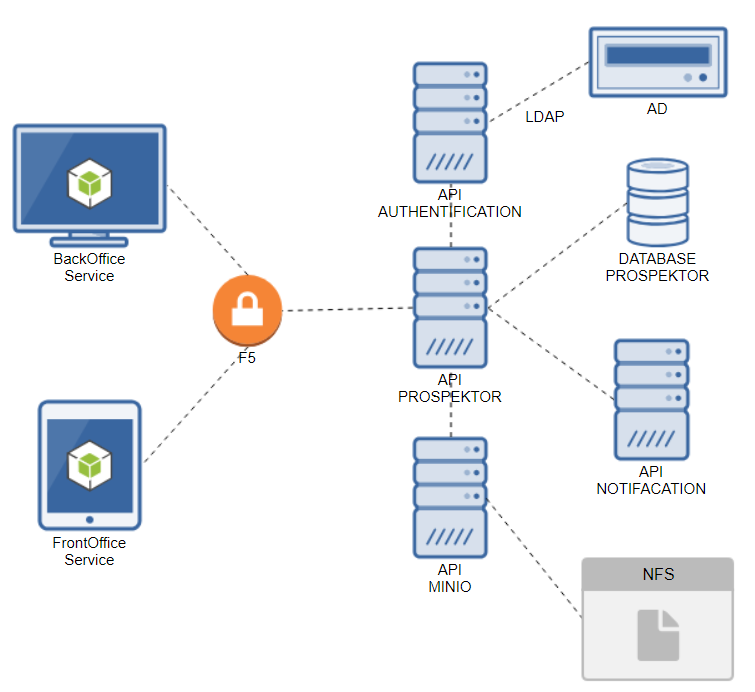
\includegraphics[width=\textwidth]{Figures/architecture.PNG}}
	\caption{\label{fig:my-label} Architecture du syst\`eme}
\end{figure}

Cette architecture est d\'efinie pour les prospecteurs et les exploitant qui vont utiliser notre application mobile.

architecture du syst\`eme est compose par:
\begin{itemize}
\item \textbf{F5 VPN} : utilise le protocole Secure Sockets Layer, une technologie d'authentification et de cryptage int\'egr\'ee \`a chaque navigateur Web, pour cr\'eer une connexion s\'ecuris\'ee et crypt\'ee sur un r\'eseau moins s\'ecuris\'e, comme Internet.
\item \textbf{MINIO} : vous permet d'utiliser un seul \gls{NAS} (comme \gls{NFS}, GlusterFS et d'autres syst\`emes de fichiers distribu\'es) en tant que syst\`eme de stockage pour plusieurs serveurs MinIO. La synchronisation entre les serveurs MinIO est prise en charge par la conception.
\item \gls{AD} est un syst\`eme bas\'e sur une base de donn\'ees qui fournit une authentification, un annuaire, une strat\'egie et d'autres services dans un environnement Windows.
\item \gls{LDAP} est un protocole d'application permettant d'interroger et de modifier des \'el\'ements dans des fournisseurs de services d'annuaire tels qu'Active Directory, qui prend en charge une forme LDAP.
\item \gls{NFS}, litt\'eralement système de fichiers en r\'eseau, est \`a l'origine un protocole qui permet \`a un ordinateur d'acc\'eder via un r\'eseau \`a des fichiers distants.
\end{itemize}

\subsection{Architecture applicative : cas g\'en\'eral pour le backend}

Pour les services Backend le choix de l'architecture applicative suit une d\'ecomposition en trois couches :
\begin{itemize}
\item Couche DAO : c'est la couche d'accd\`es aux donn\'ees persistant dans la SGBD.
\item Couche Services : impl\'emente la logique m\'etier du service, et les diff\'erentes rd\`egles de gestion qui repr\'esentent les fonctionnalit\'es du service.
\item Couche API : il permet l'encapsulation des diff\'erents services dans une API RESTfull et fournit les contr\^oleurs l'accd\`es \`a ces services.
\end{itemize}

\begin{figure}[H]
	\center{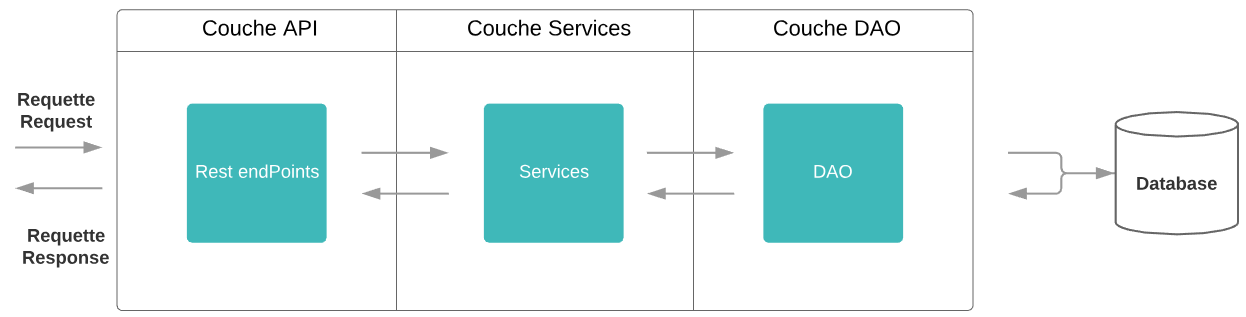
\includegraphics[width=\textwidth]{Figures/backend.PNG}}
	\caption{\label{fig:my-label} Architecture Applicative backend}
\end{figure}


\subsection{Architecture applicative : cas g\'en\'eral pour le backoffice}

L'architecture qu'on va utiliser agit comme un conteneur d'\'etat et facilite la gestion du flux de donn\'ees de notre application. Il a \'et\'e introduit en 2015 lors de la conf\'erence \textcolor{red}{ReactEurope} de \textcolor{red}{Dan Abramov}. Elle ressemble \`a l'architecture Flux et a beaucoup en commun avec elle.

\begin{figure}[H]
	\center{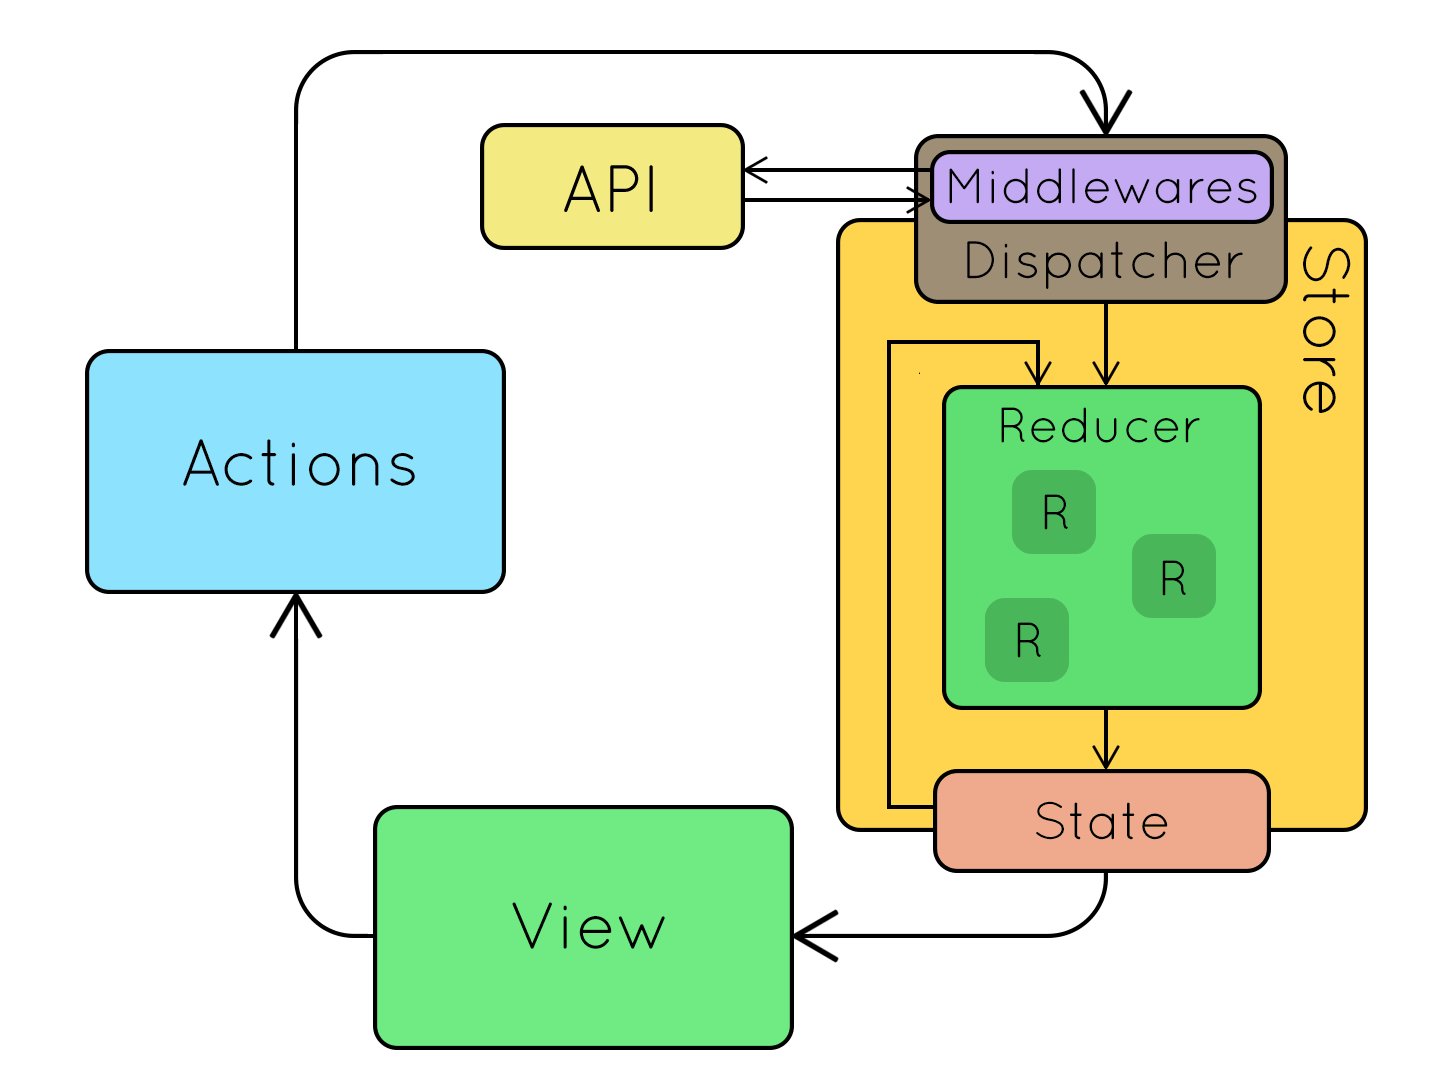
\includegraphics[width=0.6\textwidth]{Figures/backoffice.png}}
	\caption{\label{fig:my-label} Architecture Applicative backoffice}
\end{figure}

Nous avons les composants de vue qui envoient une action. La m\^eme action peut \^etre envoy\'ee par une autre partie de notre syst\`eme. Cette action est envoy\'ee non pas \`a un hub central, mais directement au store. Nous disons "store" et non "stores" car il n'y en a qu'un global. La logique qui a d\'ecid\'e comment nos donn\'ees changent vit dans des fonctions pures appel\'ees reducers. Une fois que le store re\c{c}oit une action, il demande aux reducers la nouvelle version de l'\'etat en envoyant l'\'etat actuel et l'action en question. Ensuite, de mani\`ere immuable, le reducer doit retourner le nouvel \'etat. Le store continue \`a partir de l\`a et met \`a jour son \'etat interne. Enfin, le composant c\^abl\'e au store est rendu \`a nouveau.


\subsection{Architecture applicative : cas g\'en\'eral pour le frontoffice}

Le mod\'ele de conception architecturale \gls{MVP1} est un mod\'ele de conception assez connu des d\'eveloppeurs Android. Il vous permet de d\'ecoupler la logique m\'etier de la logique de vue (Activit\'e / Fragment) en introduisant un interm\'ediaire appel\'e Pr\'esentateur.

Comme son nom l'indique, \gls{MVP1} est divis\'e en trois couches diff\'erentes.

\begin{figure}[H]
	\center{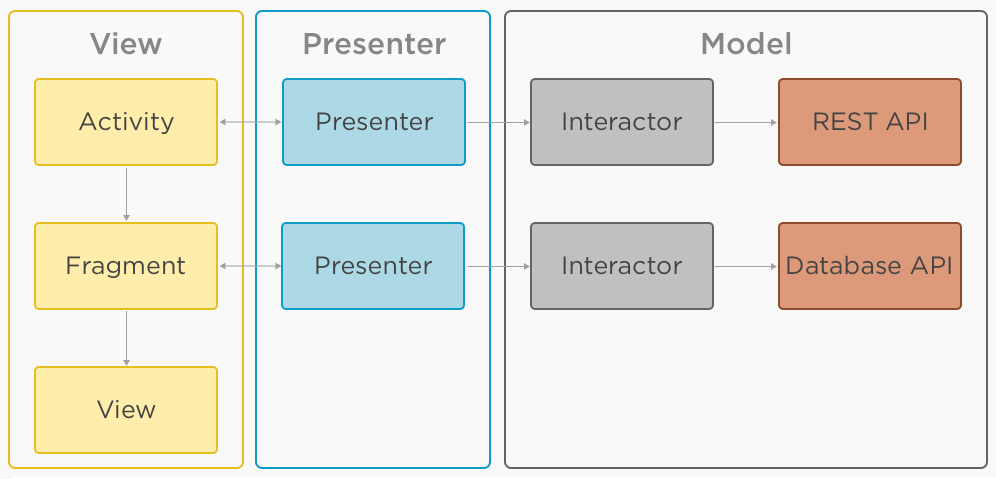
\includegraphics[width=\textwidth]{Figures/frontoffice.PNG}}
	\caption{\label{fig:my-label} Architecture Applicative frontoffice}
\end{figure}

\begin{itemize}

\item \textbf{Mod\'ele} - Comme mentionn\'e ci-dessous, o\`u est stock\'ee votre logique m\'etier et votre application de donn\'ees? Sous Android, le r\^ole d'un mod\'ele est g\'en\'eralement jou\'e par l'\gls{API} ou l'\gls{API} \gls{REST}.

Il est non seulement responsable du stockage des donn\'ees de l'application, mais \'egalement de composants contenant des responsabilit\'es pour la g\'en\'eration, l'exposition et la r\'ecup\'eration des donn\'ees.

En g\'en\'eral, toutes ces fonctionnalit\'es sont ex\'ecut\'ees en arri\'ere-plan car elles peuvent bloquer le thread d'interface utilisateur.

\item \textbf{View} - View est essentiellement une interface d'utilisateur passive qui est responsable du routage de l'action de l'utilisateur vers le pr\'esentateur. 

En g\'en\'eral, l'affichage n'est pas visible pour votre mod\'ele, \`a l'exception du POJOS et des entit\'es de l'application. Pour faire plus simplement, les vues ne communiquent pas directement avec les mod\'eles. Cependant, ils parlent aux pr\'esentateurs.

\item \textbf{Presenter} - Le pr\'esentateur est l'interm\'ediaire ou le m\'ediateur entre View et Model.

En termes g\'en\'eraux, Presenter interroge le mod\'ele et met \`a jour la vue tout en r\'epondant aux interactions de l'utilisateur.

Il surveille la fa\c{c}on dont ils sont, et ils ne peuvent pas le g\'erer.

\end{itemize}

\subsection{Les services externes}

Dans notre projet, on est besoin de trois services externes qui sont d\'ej\`a r\'ealiser par l'entit\'e \gls{DF}. La communication avec ces services se base sur les requ\^etes \gls{HTTP} \& leurs utilit\'es sont:
\begin{itemize}
\item \textbf{Service d'authentification} : permet de v\'erifier l'identit\'e d'un utilisateur, est ce qu'il est appartient au groupe \gls{OCP}.
\item \textbf{Service Minio} : permet de stocker les attachements des anomalies. On va utiliser le protocole \gls{NFS} lors du stockage.
\item \textbf{Service Notification} : permet d'envoyer des messages \gls{SMS}.
\end{itemize}


\section{\gls{ERD}}
Un certain nombre de techniques de mod\'elisation de donnd\'ees sont utilisd\'ees aujourd'hui. L'un des plus courants est le diagramme de relation d'entitd\'e (\gls{ERD}). Plusieurs notations \gls{ERD} sont disponibles. Nous avons utilis\'e la notation du Crow's Foot.

La \textbf{cardinalit\'e} et la \textbf{modalit\'e} sont les indicateurs des r\`egles de gestion entourant une relation. La cardinalit\'e fait r\'ef\'erence au nombre maximum de fois qu'une instance d'une entit\'e peut \^etre associ\'ee \`a des instances de l'entit\'e associ\'ee. La modalit\'e fait r\'ef\'erence au nombre minimum de fois qu'une instance d'une entit\'e peut \^etre associ\'ee \`a une instance de l'entit\'e associ\'ee.

\begin{table}[H]
\begin{center}
\begin{tabular}{ ll }
\hline Symbole & cardinalit\'e \\ \hline
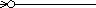
\includegraphics[width=0.2\textwidth]{Figures/0+.png}
& z\'ero ou plus \\
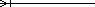
\includegraphics[width=0.2\textwidth]{Figures/1+.png}
& 1 ou plus \\
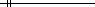
\includegraphics[width=0.2\textwidth]{Figures/11.png}
& 1 et seulement 1 \\
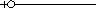
\includegraphics[width=0.2\textwidth]{Figures/01.png}
& z\'ero ou 1
\end{tabular}
\caption{Cardinalit\'e du Crow's Foot}
\end{center}
\end{table}

Le diagramme du crow's foot de notre projet prospektor est repr\'esent\'e dans le figure ci-dessous :

\begin{figure}[H]
	\center{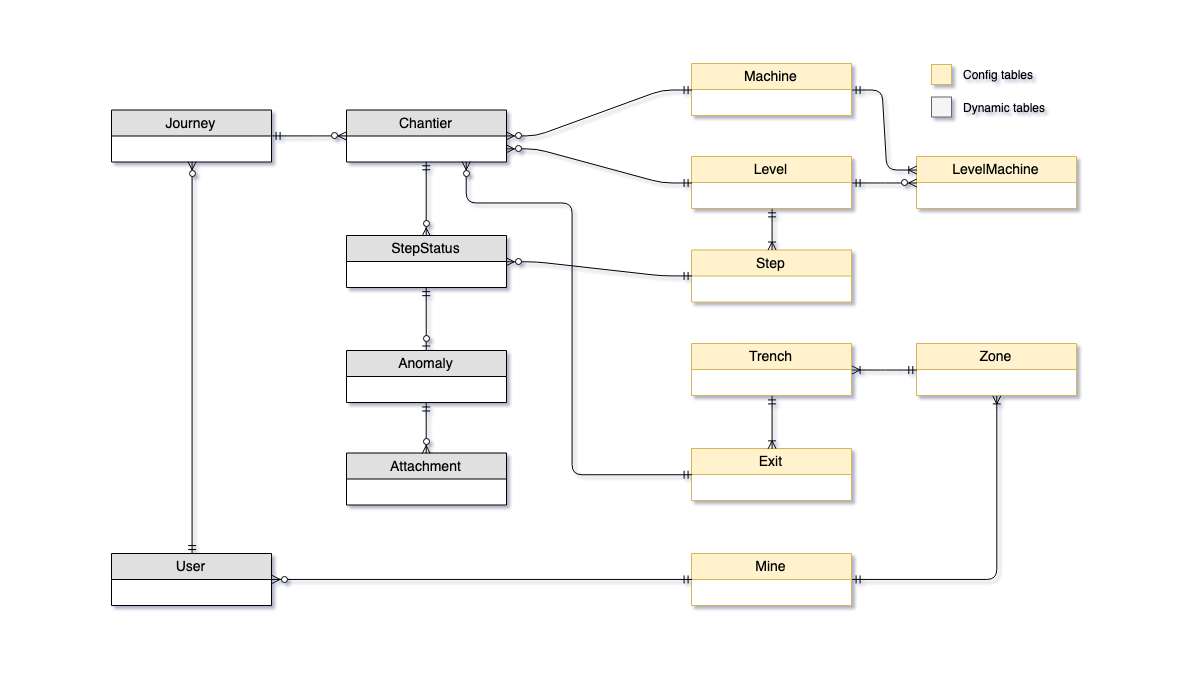
\includegraphics[width=\textwidth]{Figures/crowsfeet.PNG}}
	\caption{\label{fig:my-label} Diagramme de Crow's Foot}
\end{figure}


%\include{chap4EtudeConceptuelle}
%\include{chap5mise_en_oeuvre}
%\include{Conclusion}


% ================================== BIBLIOGRAPHIE =============================

\bibliographystyle{alpha-fr}

% =============================== INDEX DES NOTATIONS ==========================
\printindex
						
\end{document}
